\begin{frame}
    \begin{centering}
        \vskip5ex plus 1filll
        {\usebeamerfont{title page title}\usebeamercolor[fg]{title page} Wave Digital Filters\\[1.5ex]}
        \vskip0pt plus 1filll
    \end{centering}
\end{frame}

\begin{frame}{Kirchoff Domain Circuits}
    \vspace{1ex}
    \begin{itemize}
        \item Each circuit component has an impedance
        \item Each component has a voltage across its terminals and current between
        \item Components are connected in series/parallel configurations (usually)
    \end{itemize}
\end{frame}

\begin{frame}{Wave Domain Circuits}
    Circuits are made up of wave ports with incident and reflected waves.\newline\newline
    \vspace{1ex}
    Incident wave:
    \begin{equation}
        a = v + R_0 i
    \end{equation}
    Reflected wave:
    \begin{equation}
        b = v - R_0 i
    \end{equation}
\end{frame}

\begin{frame}{Wave Domain Circuits}
    \vspace{1ex}
    \begin{itemize}
        \item Each circuit component is a ``1-port element'' that inputs incident and outputs reflected wave variables
        \item Each series/parallel junction is an ``N-port adaptor'' that connects the 1-ports with a scattering junction
        \item Free parameter: port resistance
    \end{itemize}
\end{frame}

\begin{frame}{Wave Digital Filters}
    Wave Digital Filters (WDFs) were developed by Alfred Fettweis in the
    1970's and 80's.\footcite[]{Fettweis}
    \vspace{1ex}
    \begin{itemize}
        \item Digital simulation of circuits in the wave domain
        \item Discretize each circuit element independently
        \item Create binary connection tree (BCT) between circuit elements
    \end{itemize}
\end{frame}

\begin{frame}{Example Circuit: Feed-Forward Network 1}
    \begin{figure}
        \centering
        \begin{circuitikz} \draw[color=white]
            (0, 0) node[short, l=Vin] {}
            to[C, l=C3, o-] (2, 0)
            to[R, l=R7]     (3.25, 0)
            to[R, l=R19]    (6, 0)
            to[V, l=4.5V]   (6, -1.5)
            (3.5, 0) to[C, l=C16] (3.5, -1.5)
            (3.5, -1.25) node[ground]() {}
            (6.0, -1.25) node[ground]() {}
          ;
        \end{circuitikz}
        \caption{\label{fig:ff1}{\it Klon Centaur Feed-Forward Network 1 Circuit}}
    \end{figure}
\end{frame}

\begin{frame}{Example Circuit: Feed-Forward Network 1}
    \begin{figure}
        \centering
        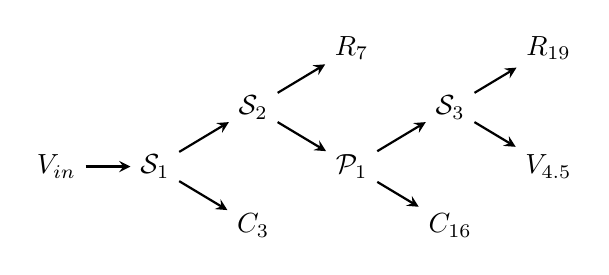
\begin{tikzpicture}[node distance=1.25cm]
            \tikzset{
                arrow/.style = {thick,->,>=stealth}
            }
            \node (Vin) {$V_{in}$};
            \node (S1)  [right of=Vin] {$\mathcal{S}_1$};
            \node (C3)  [right of=S1, below of=S1, yshift= 0.5cm] {$C_3$};
            \node (S2)  [right of=S1, above of=S1, yshift=-0.5cm] {$\mathcal{S}_2$};
            \node (R7)  [right of=S2, above of=S2, yshift=-0.5cm] {$R_7$};
            \node (P1)  [right of=S2, below of=S2, yshift= 0.5cm] {$\mathcal{P}_1$};
            \node (C16) [right of=P1, below of=P1, yshift= 0.5cm] {$C_{16}$};
            \node (S3)  [right of=P1, above of=P1, yshift=-0.5cm] {$\mathcal{S}_3$};
            \node (R19) [right of=S3, above of=S3, yshift=-0.5cm] {$R_{19}$};
            \node (V45) [right of=S3, below of=S3, yshift= 0.5cm] {$V_{4.5}$};
    
            \draw [arrow] (Vin) -- (S1);
            \draw [arrow] (S1) -- (C3);
            \draw [arrow] (S1) -- (S2);
            \draw [arrow] (S2) -- (R7);
            \draw [arrow] (S2) -- (P1);
            \draw [arrow] (P1) -- (C16);
            \draw [arrow] (P1) -- (S3);
            \draw [arrow] (S3) -- (R19);
            \draw [arrow] (S3) -- (V45);
        \end{tikzpicture}
        \caption{\label{fig:wdftree}{\it WDF tree for the Klon Centaur Feed-Forward Network 1 Circuit.
        $\mathcal{S}$ and $\mathcal{P}$ nodes refer to series and parallel adaptors respectively.}}
    \end{figure}
\end{frame}

\begin{frame}{Time-Domain Response}
    \begin{figure}
        \centering
        \includegraphics[height=2.75in]{../Paper/Figures/WDFval.png}
    \end{figure}
\end{frame}

\begin{frame}{Wave Digital Filters}
    \begin{columns}
        \begin{column}{0.5\linewidth}
            \hspace{-1ex}
            Advantages:
            \vspace{1ex}
            \begin{itemize}
                \itemsep0.5em
                \item Modularity: circuit elements and topology can be alterred on-the-fly
                \item Each element can be discretized with a different conformal map
                % \item Requires very little prior knowledge
            \end{itemize}
        \end{column}
        \begin{column}{0.5\linewidth}
            \hspace{-1ex}
            Disadvantages:
            \vspace{1ex}
            \begin{itemize}
                \itemsep0.5em
                \item Cannot model circuits with multiple nonlinearities or $\mathcal{R}$-type topologies
                \item These types of circuits can be modelled using $\mathcal{R}$-adaptors,
                but with an increase in complexity
            \end{itemize}
        \end{column}
    \end{columns}
\end{frame}

\begin{frame}{Wave Digital Filters}
    More information:
    \vspace{1ex}
    \begin{itemize}
        \itemsep0.75em
        \item Alfred Fettweis, ``Wave Digital Filters: Theory and Practice'',
        \emph{Proceedings of the IEEE}, vol. 74, no. 2, 1986
        \begin{itemize}
            \item Original reference for deriving WDF formalism
        \end{itemize}

        \item Kurt Werner, \emph{Virtual Analog Modeling of Audio Circuitry Using Wave Digital Filters},
        PhD. Thesis, Stanford University, 2016
        \begin{itemize}
            \item Great reference for deriving WDFs, including more recent advancements
            \item Expands WDFs to handle $\mathcal{R}$-type topologies and multiple nonlinearities
        \end{itemize}
    \end{itemize}
\end{frame}

\begin{frame}{Wave Digital Filters}
    More information:
    \vspace{1ex}
    \begin{itemize}
        \itemsep0.75em
        \item Fran\c{c}ois Germain, \emph{Non-oversampled physical modeling for virtual analog simulation},
        PhD. Thesis, Stanford University, 2019
        \begin{itemize}
            \item Example of independently discretizing circuit elements with Alpha Transform
        \end{itemize}

        \item Jingjie Zhang and Julius Smith, ``Real-time Wave Digital Simulation of
        Cascaded Vacuum Tube Amplifiers Using Modified Blockwise Method'',
        \emph{Proc. of the 21st International Conference on Digital Audio Effects}, 2018
        \begin{itemize}
            \item Real-time simulation of an impressively large circuit
        \end{itemize}
    \end{itemize}
\end{frame}
